\section{Auswertung}
\label{sec:Auswertung}

In \ref{tab:Tabelle} sind die Stromstärken, die das Intensitätsmessgerät bei den beiden Einzelspalten und bei dem Doppelspalt gemessen hat, gegen $x$ aufgetragen.
$x$ ist hier die Skala bei der Verschiebeapparatur des Intensitätsmessgerätes, wobei es bei $x=\qty{25}{\milli\meter}$ mittig zum Laser liegen sollte.

\begin{table}[http]
  \centering
  \caption{In dieser Tabelle ist die gemessene Stromstärke, die von dem Intensitätsmessgerät ausgegeben wird, in Abhängigkeit zur Verschiebung des Messgerätes in x Richtung eingetragen.
  Dabei ist $I_S1$ die Stromstärke für den ersten Einzelspalt, $I_S2$ die für den zweiten Einzelspalt und $I_DS$ die für den Doppelspalt.}
  \label{tab:Tabelle}
  \sisetup{table-format=1.1, per-mode=reciprocal}
  \begin{minipage}[t]{0.4\linewidth}
    \begin{tblr}[t]{
      colspec = {S[table-format=2.1] S[table-format=1.2] S[table-format=2.2] S[table-format=2.1]},
      row{1} = {guard, mode=math},
    }
    \toprule
    x \mathbin{/} \unit{\volt} & I_S1 \mathbin{/} \unit{\nano\ampere} & I_S2 \mathbin{/} \unit{\nano\ampere} & I_DS \mathbin{/} \unit{\nano\ampere} \\
    \midrule
   0.0 &   0.32   &   0.32  & 1.4 \\
   1.0 &   0.32   &   0.36  & 1.0 \\
   2.0 &   0.32   &   0.40  & 1.2 \\
   3.0 &   0.32   &   0.44  & 1.8 \\
   4.0 &   0.32   &   0.50  & 1.8 \\
   5.0 &   0.34   &   0.70  & 1.8 \\
   6.0 &   0.40   &   1.00  & 1.8 \\
   7.0 &   0.52   &   1.40  & 1.4 \\
   8.0 &   0.66   &   1.60  & 2.0 \\
   9.0 &   0.82   &   1.60  & 3.0 \\
  10.0 &   1.00   &   1.40  & 3.2 \\
  11.0 &   1.20   &   1.20  & 4.0 \\
  12.0 &   1.20   &   1.40  & 4.4 \\
  13.0 &   1.40   &   2.00  & 4.8 \\
  14.0 &   1.40   &   2.40  & 4.2 \\
  15.0 &   1.40   &   2.80  & 3.4 \\
  16.0 &   1.40   &   2.60  & 4.4 \\
  17.0 &   1.60   &   2.40  & 7.0 \\
  18.0 &   1.80   &   2.20  & 9.0 \\
  19.0 &   2.20   &   2.60  & 10.0 \\
  20.0 &   2.80   &   3.00  & 12.0 \\
  20.5 &   3.20   &   3.20  & 26.0 \\
  21.0 &   3.40   &   3.80  & 20.0 \\
  21.5 &   3.80   &   4.40  & 24.0 \\
  22.0 &   4.00   &   6.00  & 34.0 \\
  22.5 &   4.00   &   7.80  & 20.0 \\
  23.0 &   4.20   &  10.00  & 42.0 \\
  23.5 &   4.20   &  14.00  & 28.0 \\
  24.0 &   4.20   &  16.00  & 32.0 \\
  24.5 &   4.00   &  16.00  & 36.0 \\
  25.0 &   3.80   &  18.00  & 22.0 \\

    \bottomrule
  \end{tblr}
\end{minipage}
\hfill
\begin{minipage}[t]{0.4\linewidth}
    \begin{tblr}[t]{
      colspec = {S[table-format=2.1] S[table-format=1.2] S[table-format=2.2] S[table-format=2.1]},
      row{1} = {guard, mode=math},
    }
    \toprule
    x \mathbin{/} \unit{\volt} & I_S1 \mathbin{/} \unit{\nano\ampere} & I_S2 \mathbin{/} \unit{\nano\ampere} & I_DS \mathbin{/} \unit{\nano\ampere} \\
    \midrule
    25.5 &   3.60   &  16.00  & 32.0 \\
    26.0 &   3.20   &  16.00  & 20.0 \\
    26.5 &   3.00   &  14.00  & 22.0 \\
    27.0 &   2.80   &  12.00  & 20.0 \\
    27.5 &   2.40   &   9.40  & 14.0 \\
    28.0 &   2.00   &   7.80  & 18.0 \\
    28.5 &   2.00   &   6.80  & 14.0 \\
    29.0 &   1.80   &   6.00  & 12.0 \\
    29.5 &   1.60   &   5.80  & 14.0 \\
    30.0 &   1.40   &   5.20  & 10.0 \\
    31.0 &   1.20   &   4.20  & 12.0 \\
    32.0 &   1.20   &   3.00  & 10.0 \\
    33.0 &   1.40   &   2.40  & 7.0 \\
    34.0 &   1.40   &   2.20  & 6.2 \\
    35.0 &   1.60   &   2.00  & 6.4 \\
    36.0 &   1.60   &   1.80  & 6.2 \\
    37.0 &   1.60   &   2.00  & 5.6 \\
    38.0 &   1.40   &   2.20  & 7.2 \\
    39.0 &   1.40   &   2.00  & 8.8 \\
    40.0 &   1.20   &   1.60  & 7.0 \\
    41.0 &   1.00   &   1.20  & 4.4 \\
    42.0 &   1.00   &   1.20  & 4.8 \\
    43.0 &   0.74   &   1.20  & 4.4 \\
    44.0 &   0.68   &   1.00  & 2.6 \\
    45.0 &   0.66   &   1.00  & 2.0 \\
    46.0 &   0.70   &   1.00  & 2.2 \\
    47.0 &   0.76   &   1.00  & 2.4 \\
    48.0 &   0.82   &   0.84  & 2.2 \\
    49.0 &   0.86   &   0.70  & 2.0 \\
    50.0 &   0.86   &   0.72  & 2.4 \\
    \bottomrule
  \end{tblr}
\end{minipage}
\end{table}

\subsection{Einzelspalt 1}
In Abbildung \ref{fig:Spalt1} wird $I_1$ gegen $\varphi$ aufgetragen, wobei 
\begin{equation}
  \varphi=x/L
\end{equation}
ist.
Mit Formel \ref{eqn:Intensität} wird eine Ausgleichsfunktion an die Messwerte angelegt. 

\begin{figure}[H]
  \centering
  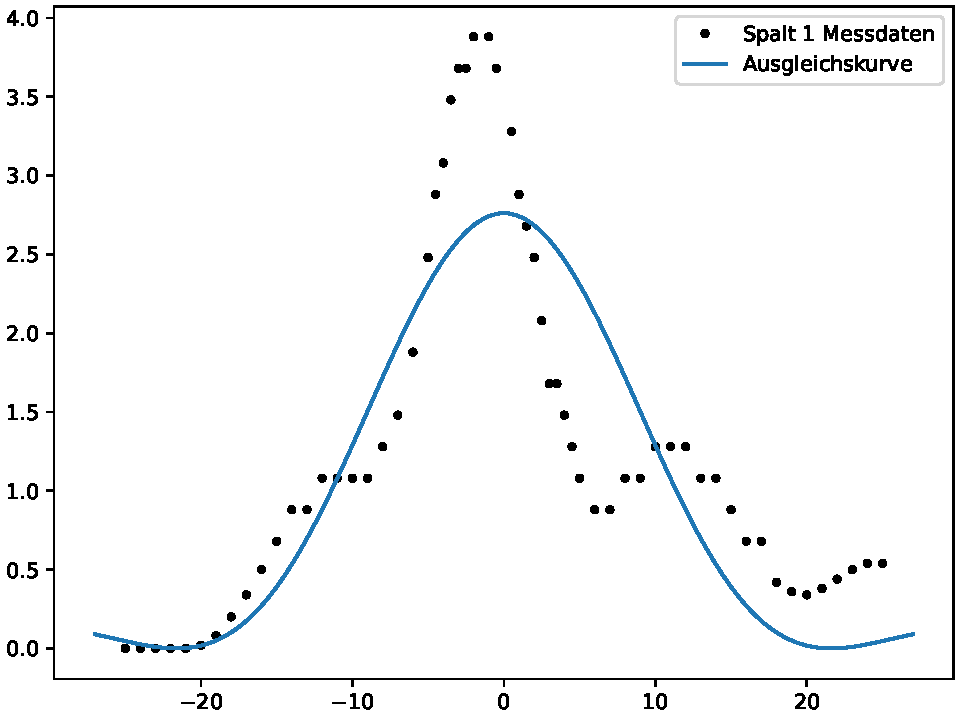
\includegraphics{plot.pdf}
  \caption{Hier ist $I_1$ in Abhängigkeit zu $\varphi$ aufgetragen.}
  \label{fig:Spalt1}
\end{figure}

Mithilfe der Ausgleichsfunktion lässt sich ein Wert für die Spaltbreite ermitteln.
Dabei ist $b_1=\qty{2.9(0.2)e-5}{\meter}$. 

\subsection{Einzelspalt 2}
Für den zweiten Spalt ist die in \ref{fig:Spalt1} $I_2$ gegen $\varphi$ aufgezeichnet.
Die Konstruktion der Ausgleichsfunktion wird abnalog zu Spalt 1 durchgeführt.

\begin{figure}[H]
  \centering
  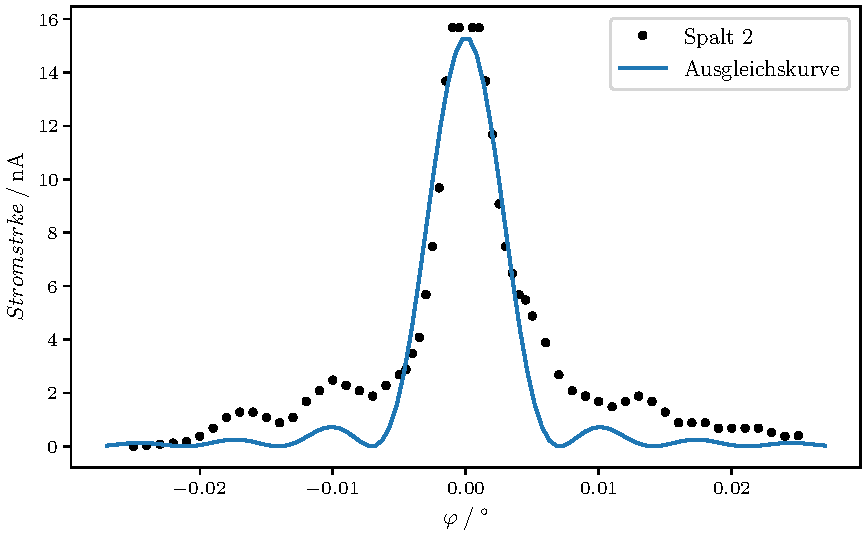
\includegraphics{plot1.pdf}
  \caption{In dieser Abbildung wird $I_2$ abhängig von $\varphi$ aufgezeichnet.}
  \label{fig:Spalt2}
\end{figure}

Hier ergibt sich ein Wert von $b_2=\qty{9.01(0.35)e-5}{\meter}$.

\subsection{Doppelspalt}

In der Abbildung \ref{fig:Doppelspalt} wird der Verlauf von $I_DS$ gegenüber $\varphi$ abgebildet.
Hier muss für die Ausgleichsfunktion die Formel \ref{eqn:Intensität2} verwendet werden.

\begin{figure}[H]
  \centering
  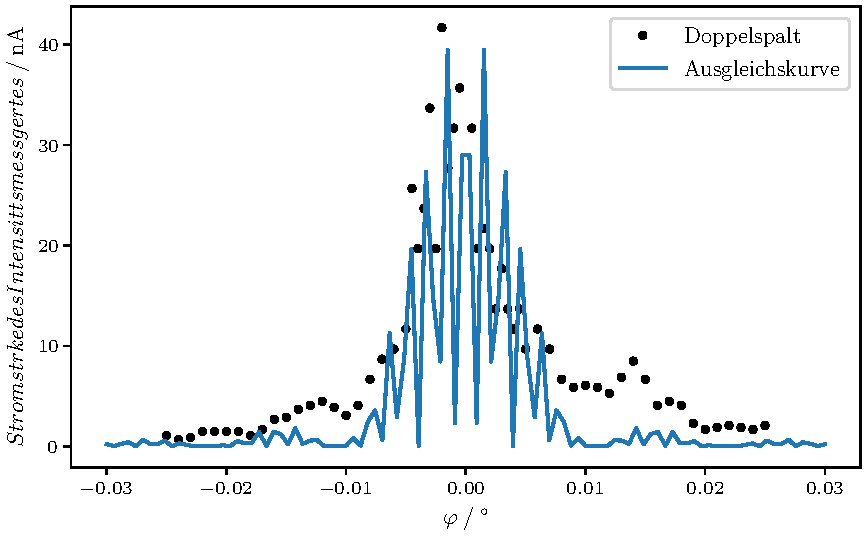
\includegraphics{plot2.pdf}
  \caption{Hier sind die Werte von $I_DS$ zu den entsprechenden Werten von $\varphi$ aufgetragen.}
  \label{fig:Doppelspalt}
\end{figure}

\noindent durch die Ausgleichsfunktion wird ein Wert von $b_{DS}=\qty{5.9(0.8)e-5}{\meter}$ berechnet.
Der Spaltabstand ist dabei $s_{DS}=\qty{4.02(0.06)e-4}{\meter}$.
